\documentclass{beamer}
\usetheme{}
\usecolortheme{dolphin}           
\useinnertheme{circles}
\setbeamertemplate{itemize items}[default]
\setbeamertemplate{enumerate items}[default]
\usepackage[T1]{fontenc}
\usepackage[utf8]{inputenc}
\usepackage{lmodern}
\usepackage{amsmath}
\usepackage{booktabs} 
\usepackage{graphicx}        
\usepackage{array}
\usepackage{color}
\usepackage{textcomp}
\usepackage{epstopdf}
\makeatletter
\def\zapcolorreset{\let\reset@color\relax\ignorespaces}
\def\colorrows#1{\noalign{\aftergroup\zapcolorreset#1}\ignorespaces}
\makeatother
\graphicspath{{/home/swl/Dropbox/ucd/international_trade/tex/}} 
\setbeamertemplate{navigation symbols}{}

%--------------------------------------
%%%% DETAILS TITLE PAGE %%%%
%--------------------------------------
\title{International trade: trade issues}
\author{School of Economics, University College Dublin}
\date{Autumn 2017}
\begin{document}
%--------------------------------------
%%%% TITLE SLIDE %%%%
%--------------------------------------
\begin{frame}
\titlepage  
\end{frame}
%--------------------------------------

%--------------------------------------
\begin{frame}
  There are a number of issues related to international trade that we haven't discussed in detail so far such as
  \begin{enumerate}
    \item Effect on inequality
    \item Dumping    
    \item Labour standards
    \item Effect on environment
  \end{enumerate}  
\end{frame}
%--------------------------------------


%--------------------------------------
\begin{frame}
  Some people oppose trade liberalisation because of the effect it has on income, given that trade liberalisation will increase the relative returns of the abundant factor, which often is land or capital.
  \begin{itemize}
    \item i.e. not the workers, proletariat, etc.
  \end{itemize}  
\end{frame}
%--------------------------------------

%--------------------------------------
\begin{frame}
Concerning trade and income inequality, following the HO-model we would expect to observe two things
\begin{enumerate}
  \item Capital gains in developed countries
  \item Labour gains in developing countries
\end{enumerate}
\medskip
This means that trade will increase inequality in industrialised states and reduce it in developing countries.
\end{frame}
%--------------------------------------

%--------------------------------------
\begin{frame}
  \begin{figure}
    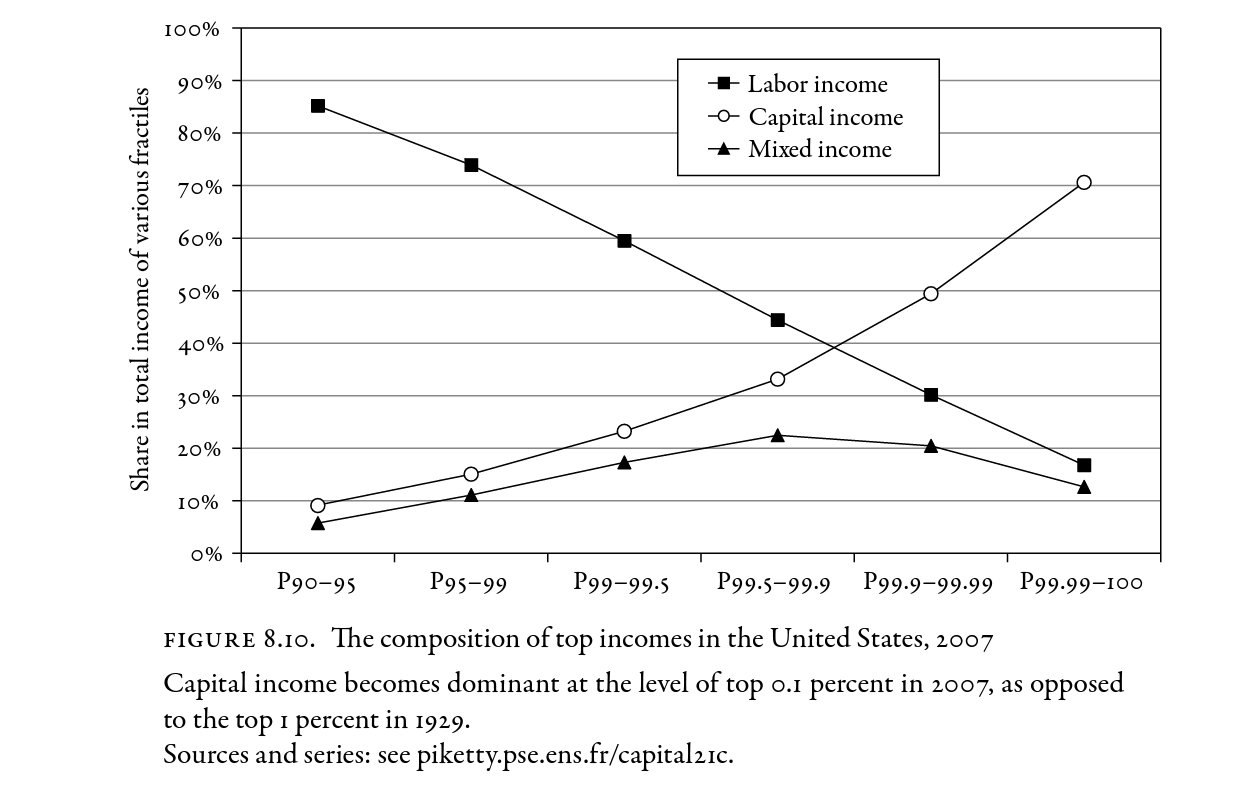
\includegraphics[scale=.2]{piketty.png}
  \end{figure}
\end{frame}
%--------------------------------------

%--------------------------------------
\begin{frame}
  \begin{figure}
    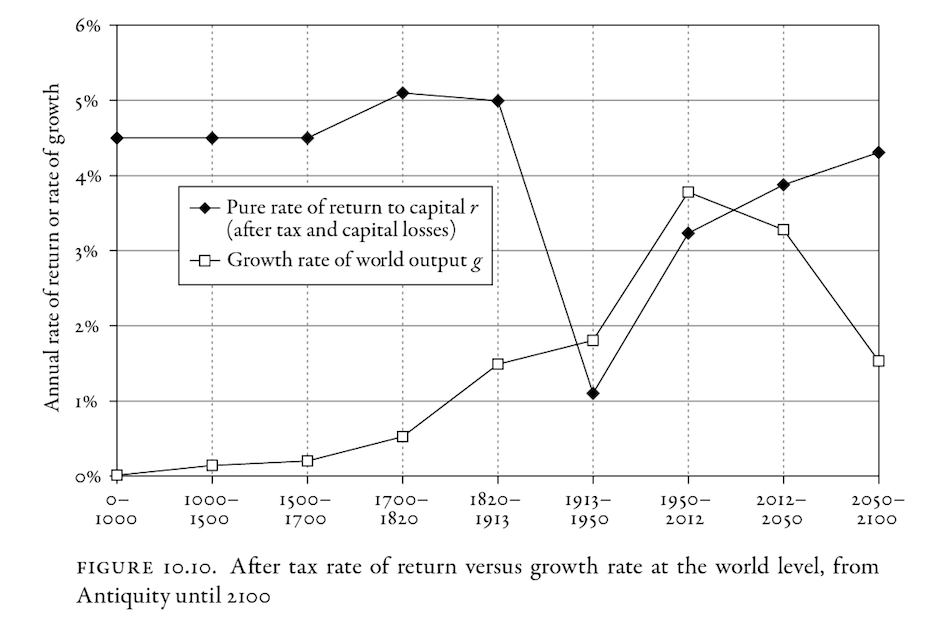
\includegraphics[scale=.2]{piketty2.png}
  \end{figure}
\end{frame}
%--------------------------------------

%--------------------------------------
\begin{frame}
  \begin{figure}
    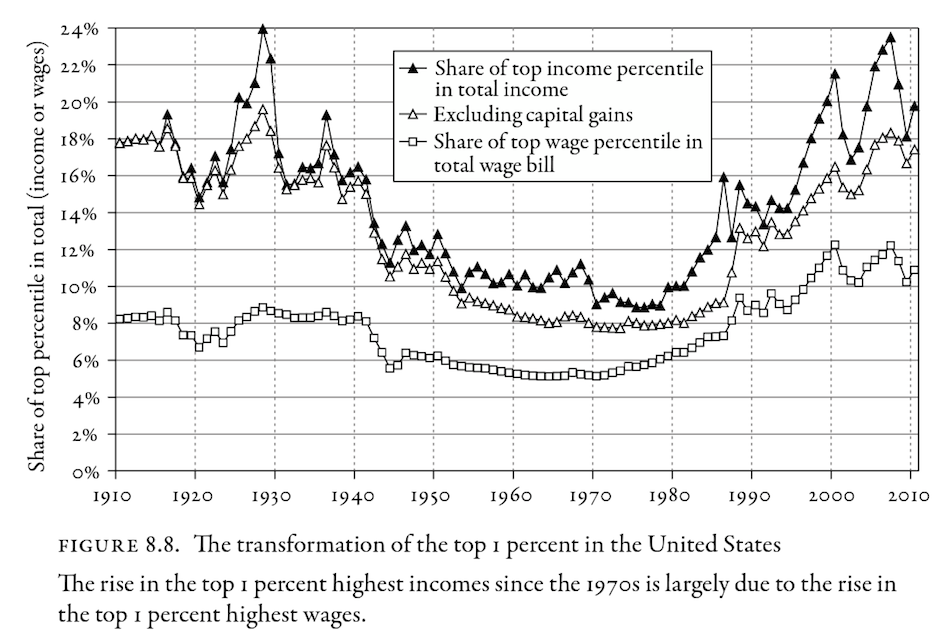
\includegraphics[scale=.2]{piketty3.png}
  \end{figure}
\end{frame}
%--------------------------------------

%--------------------------------------
\begin{frame}
  What does the literature have to say on the topic of trade and income inequality? 
 \begin{itemize}
    \item Globalisation linked to reduction in inequality between countries but not necessarily within 
    \item Wages of high-skilled workers in developed countries have increased while those for unskilled labour have fallen
  \end{itemize}
\end{frame}
%--------------------------------------

%--------------------------------------
\begin{frame}
  \begin{figure}
    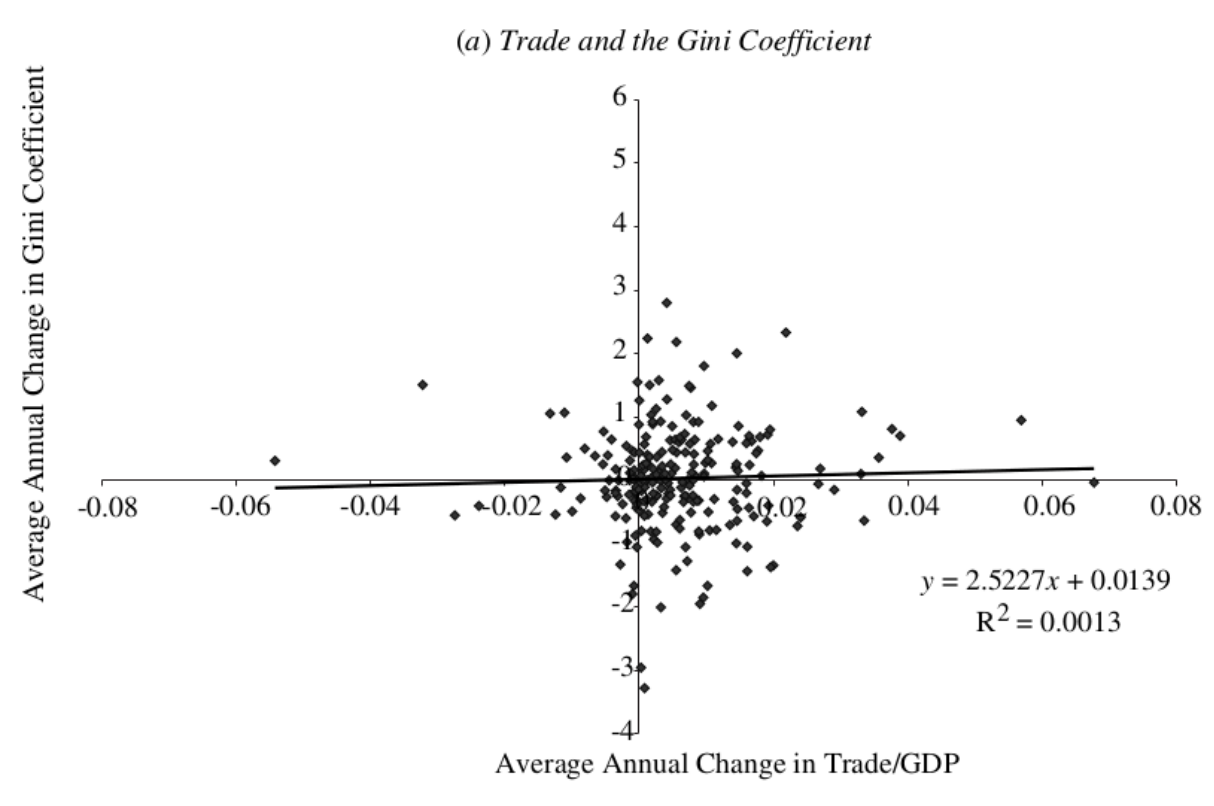
\includegraphics[scale=.7]{trade_gini.png}
  \end{figure}
  Dollar \& Kraay, 2004, "Trade, Growth, and Poverty"
\end{frame}
%--------------------------------------

%--------------------------------------
\begin{frame}
  \begin{figure}
    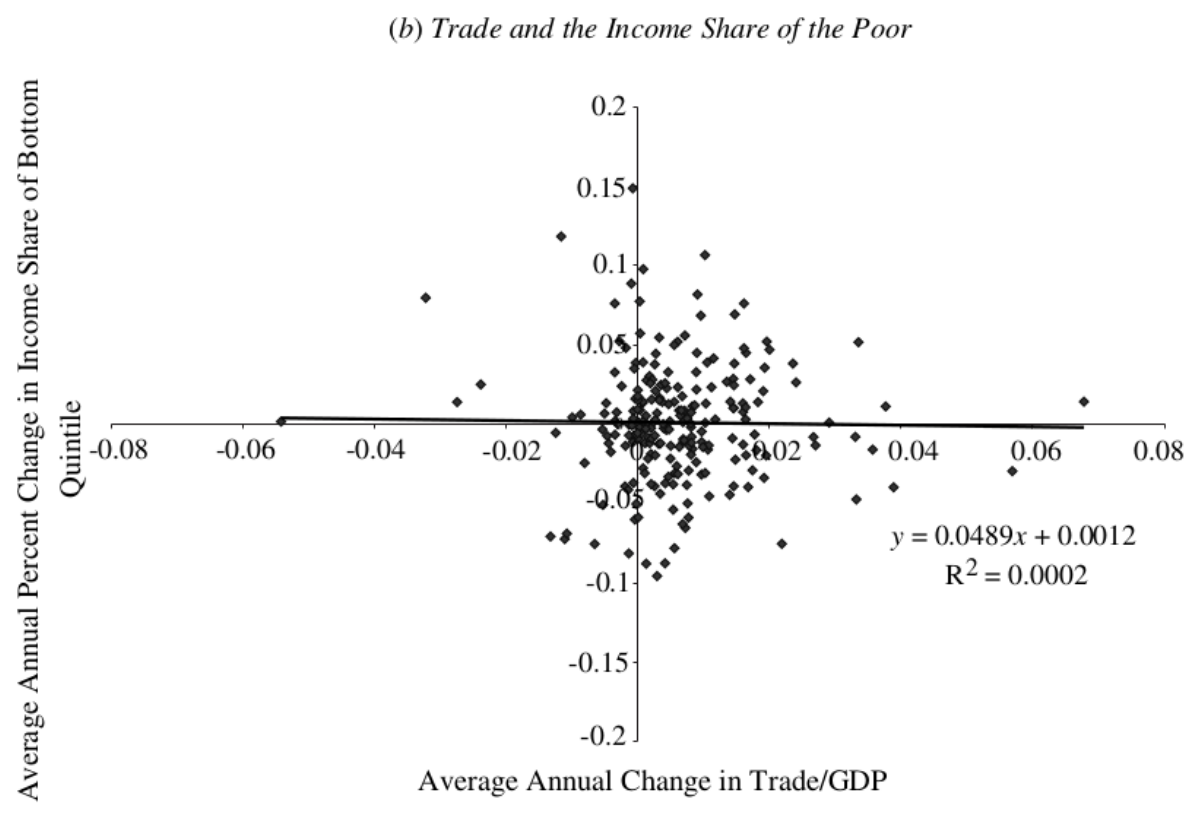
\includegraphics[scale=.7]{trade_gini2.png}
  \end{figure}
  Dollar \& Kraay, 2004, "Trade, Growth, and Poverty"
\end{frame}
%--------------------------------------

%--------------------------------------
\begin{frame}
  One negative side effect of free trade is \textbf{dumping}, which can be defined as
  \begin{quote}
    An exporting firm setting an export price below its domestic market price plus all per-unit trade costs
  \end{quote}
  \medskip
  This is an example of price discrimination 
  \begin{itemize}
    \item Firm can charge different prices to different consumers
  \end{itemize}  
\end{frame}
%--------------------------------------

%--------------------------------------
\begin{frame}
  Dumping requires two market conditions
  \begin{enumerate}
    \item Imperfect competition
    \item Market segmentation
  \end{enumerate}
  \medskip
  In international trade these arise due to fact that markets aren't perfectly integrated as a result of trade costs
  \begin{itemize}
    \item Protectionism, such as export subsidies, also leads to market distortions
  \end{itemize}
\end{frame}
%--------------------------------------

%--------------------------------------
\begin{frame}
  What is the rationale behind dumping?\\
  Let's assume that a country is faced with two different demand functions
  \begin{enumerate}
    \item Domestic 
    \item International
  \end{enumerate}
  \medskip
  Due to transport costs and home bias, domestic firms will usually have a larger market share than foreign firms.  
\end{frame}
%--------------------------------------

%--------------------------------------
\begin{frame}
  \begin{figure}
    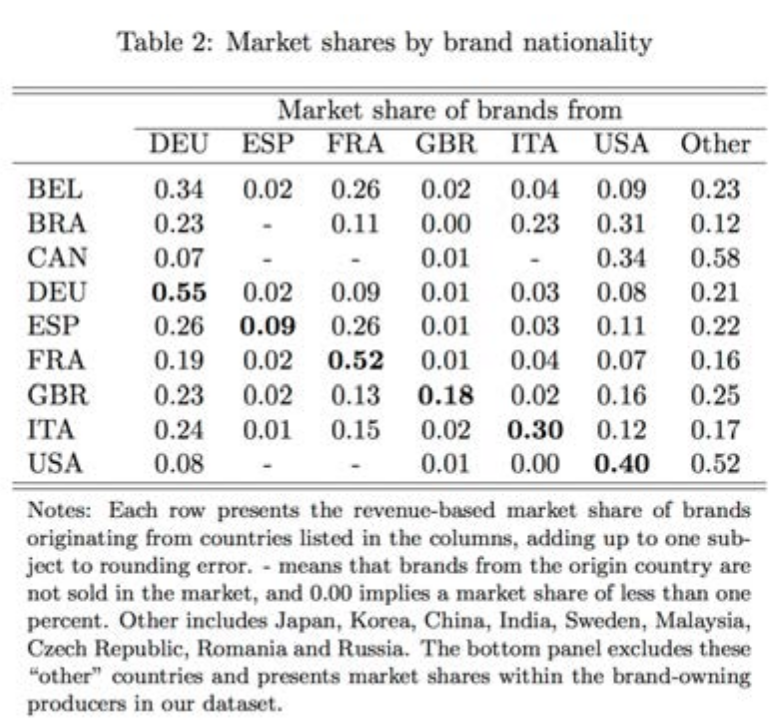
\includegraphics{market_share.png}
  \end{figure}
\end{frame}
%--------------------------------------

%--------------------------------------
\begin{frame}
Now suppose that a larger market share is associated with a demand function that is less responsive to price changes.
  \begin{itemize}
    \item This means that firms will have lower markups and lower prices in foreign markets    
  \end{itemize}  
  \medskip
  i.e. an exporting firm will lower the markup for the export market due to higher marginal costs
\end{frame}
%--------------------------------------

%--------------------------------------
\begin{frame}
 Let's consider a single good which is sold at the domestic market for $p$ and $p^*$ is the price in the foreign market. 
 The firm will face higher marginal costs in the export market adding $c+t$ to the price. 
 We get
 \begin{align*}
   p&-c\\
   p^*&-(c+t)
 \end{align*}
 Given that
 \begin{align*}
  p^*-t < p
 \end{align*}
 the export price will be lower than the domestic price.
\end{frame}
%--------------------------------------

%--------------------------------------
\begin{frame}
  Dumping is natural firm behaviour but it is considered as unfair and potentially harmful to domestic producers.
  \begin{itemize}
    \item Anti-dumping laws can be used to discriminate against imports in market
  \end{itemize}
  \medskip
  Some dumping behaviour is facilitated by subsidies such as in China for steel, 
  \begin{itemize}
    \item Chinese firms have preferential lending rates and lower energy charges
  \end{itemize}  
\end{frame}
%--------------------------------------

%--------------------------------------
\begin{frame}
  \begin{figure}
    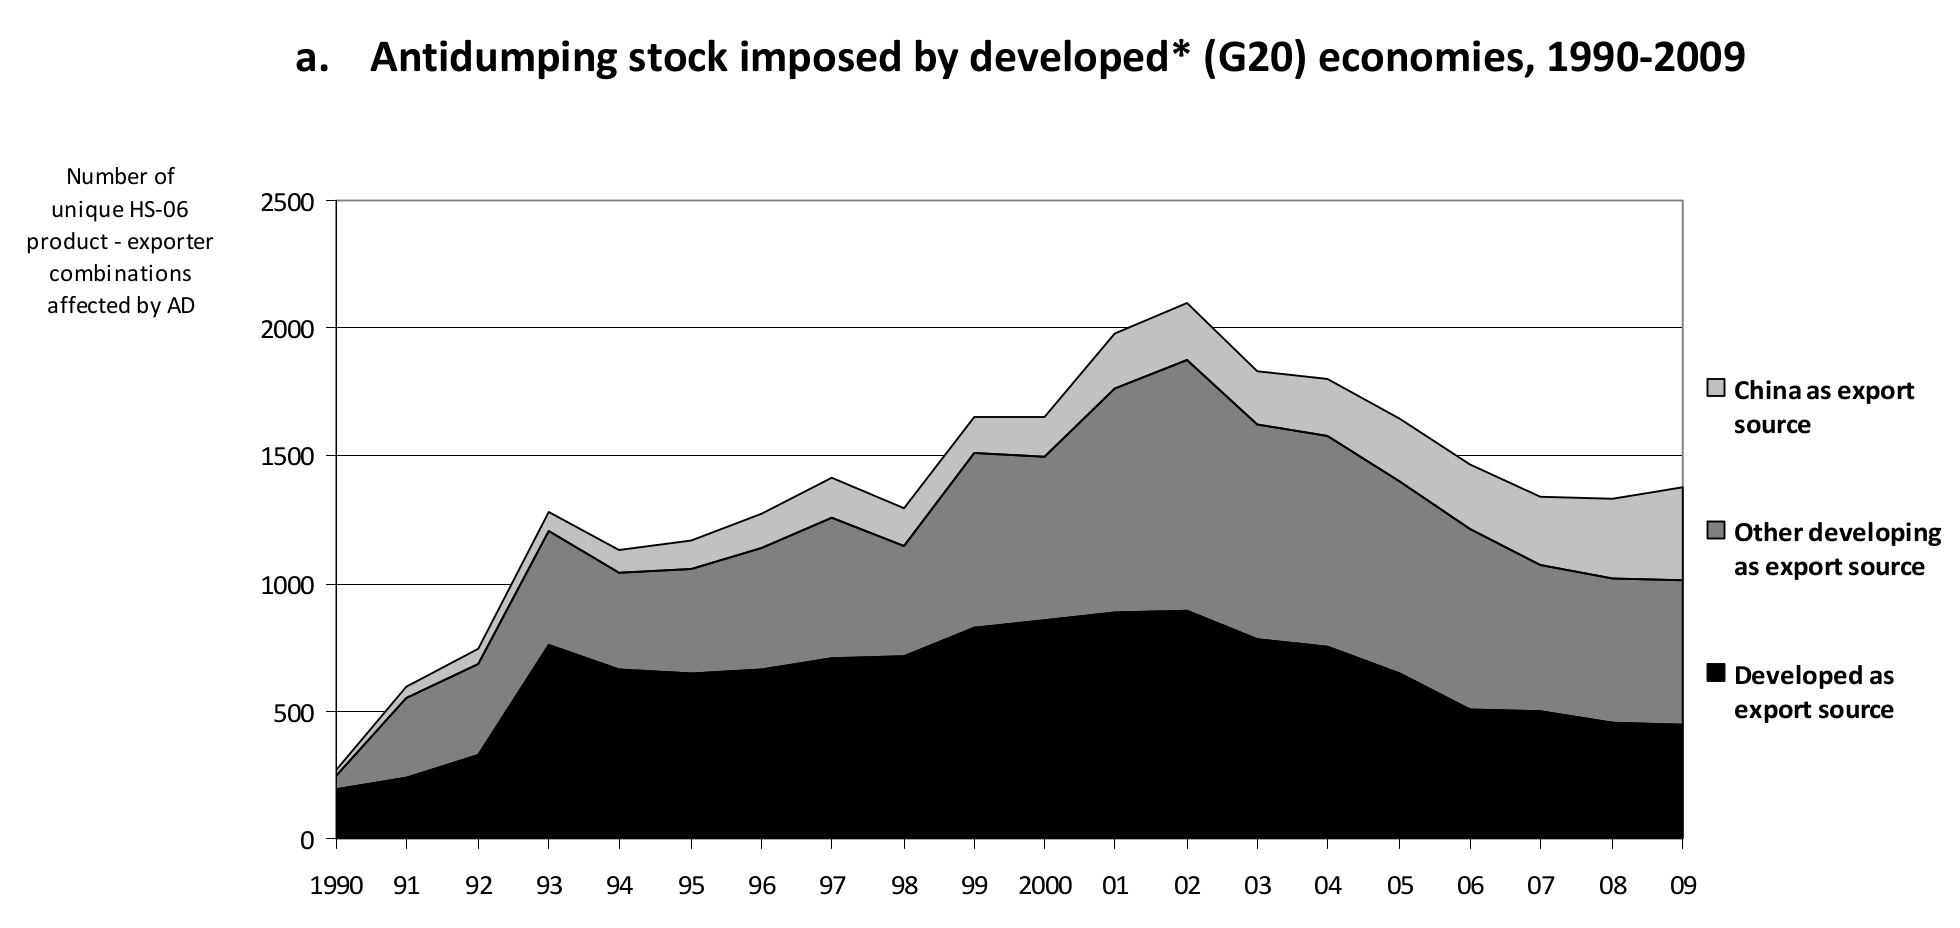
\includegraphics[scale=.7]{anti_dumping.png}
  \end{figure}
  "Taking Stock of Antidumping, Safeguards and Countervailing Duties, 1990-2009"
\end{frame}
%--------------------------------------

%--------------------------------------
\begin{frame}
  \begin{figure}
    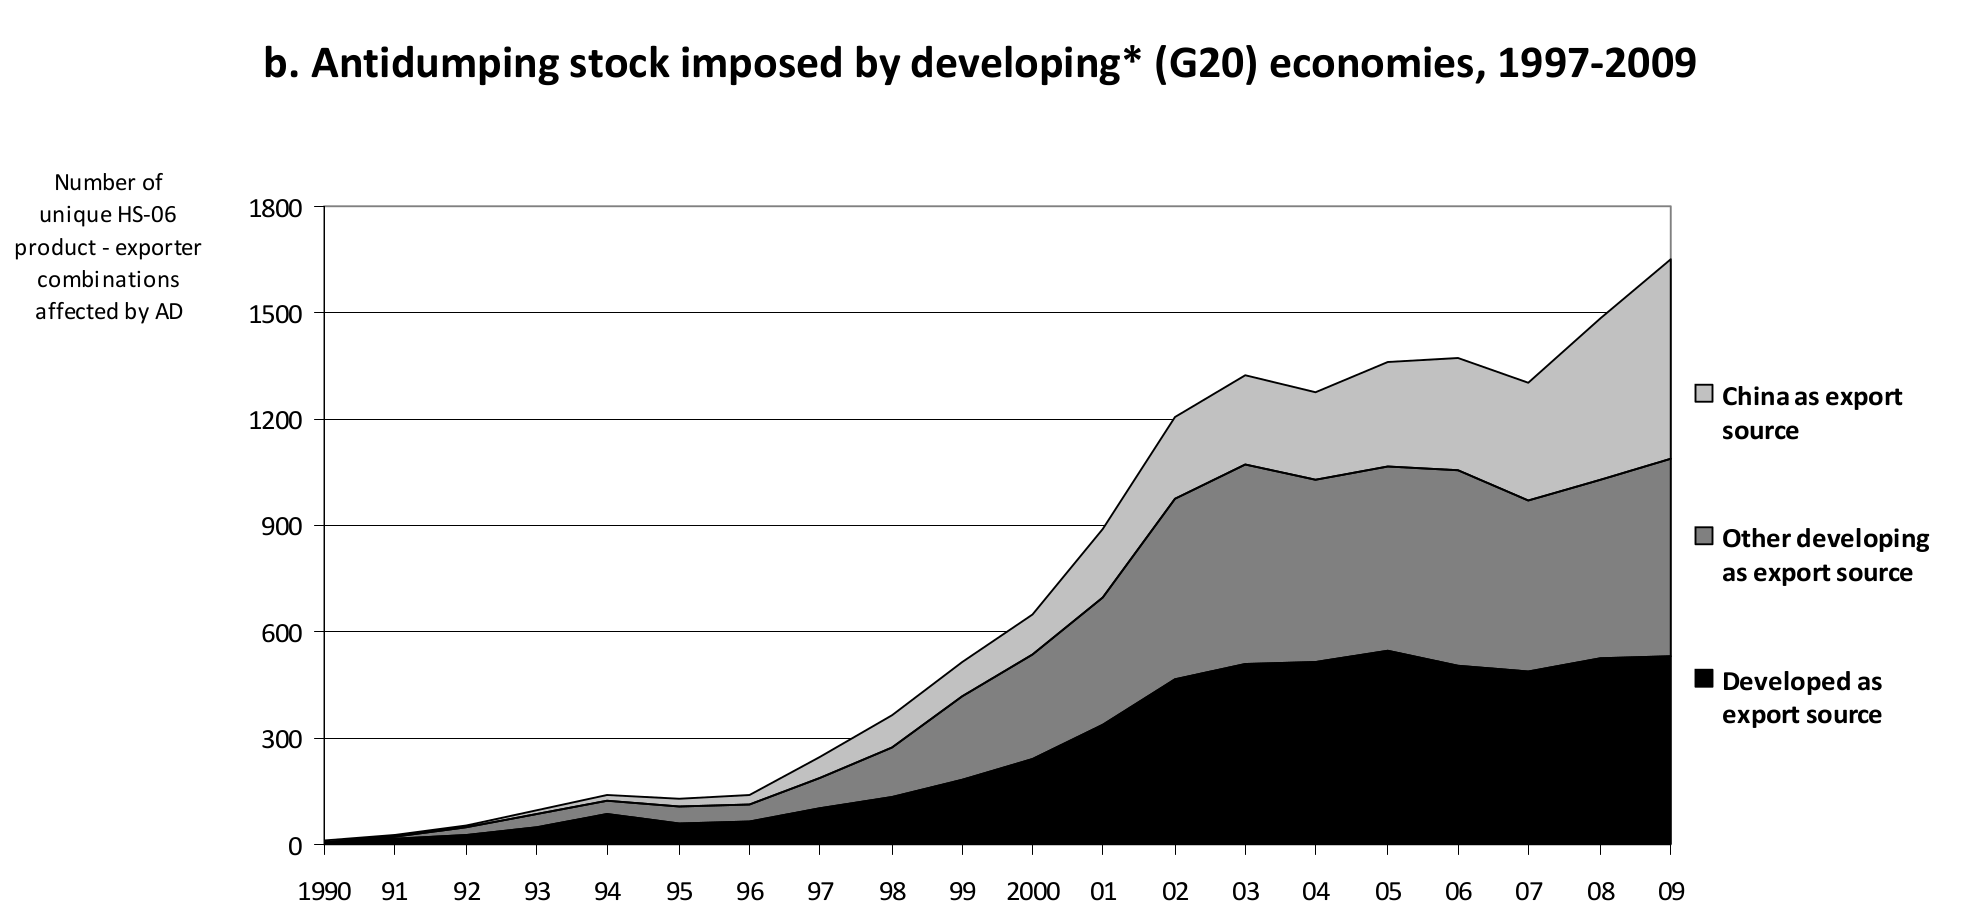
\includegraphics[scale=.7]{anti_dumping2.png}
  \end{figure}
  "Taking Stock of Antidumping, Safeguards and Countervailing Duties, 1990-2009"
\end{frame}
%--------------------------------------

%--------------------------------------
\begin{frame}
  There are two other main issues concerning trade
  \begin{enumerate}
    \item Relation to labour standards
    \item Effect on environment    
  \end{enumerate}
  \medskip
  Does trade harm the environment and do labour standards and international competition have a negative effect?
  \begin{itemize}
    \item Note that in both cases weaker environmental regulations and less strict labour laws can be a comparative advantage
  \end{itemize}
\end{frame}
%--------------------------------------

%--------------------------------------
\begin{frame}
  \begin{figure}
    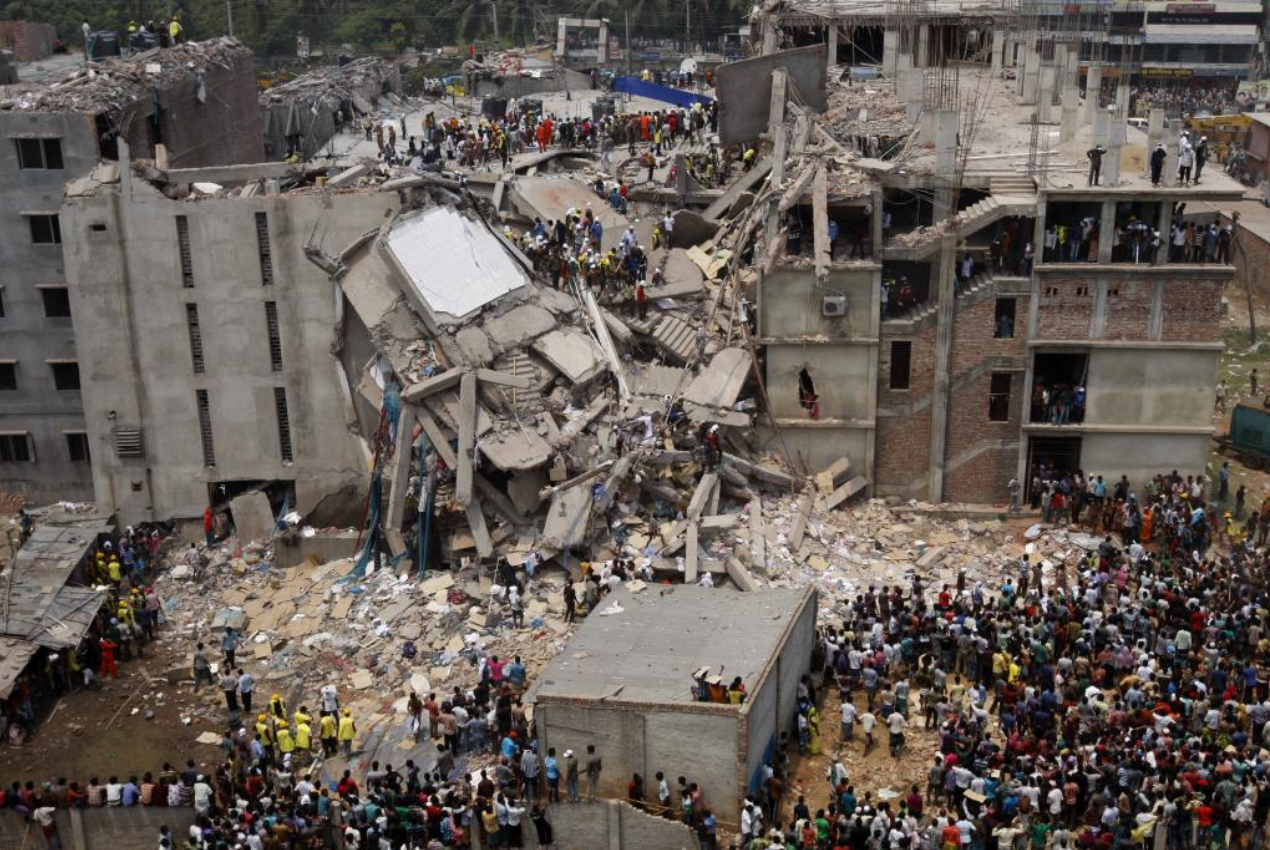
\includegraphics{rana_plaza.png}
  \end{figure}
\end{frame}
%--------------------------------------

%--------------------------------------
\begin{frame}
  In 2013 the Rana Plaza garment factory collapsed killing 1,129 people. 
  \begin{itemize}
    \item Building was converted to industrial use
    \item Little regard for workers safety, as safety precautions cost money
  \end{itemize}
  \medskip
  In response labour organisations, NGOs, and retailers signed the Accord on Fire and Building Safety in Bangladesh aimed at maintaining minimum safety standards in textile industry.
  \begin{itemize}
    \item Retailers don't check if firms comply, which isn't their job
  \end{itemize}
\end{frame}
%--------------------------------------

%--------------------------------------
\begin{frame}
  \begin{figure}
    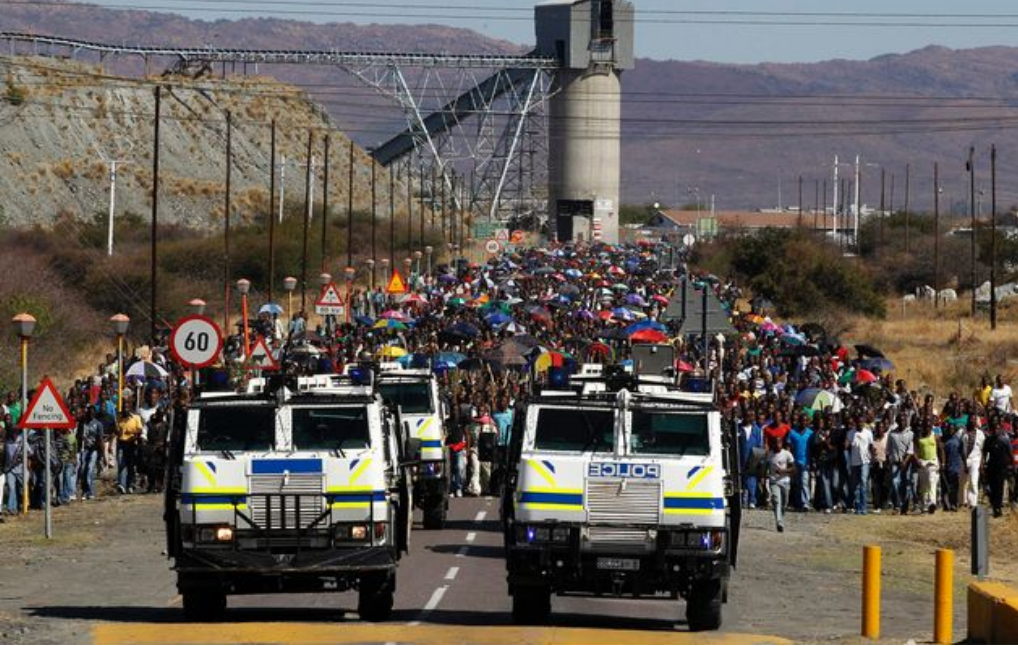
\includegraphics{mining_strike.png}
  \end{figure}
\end{frame}
%--------------------------------------

%--------------------------------------
\begin{frame}
  \begin{figure}
    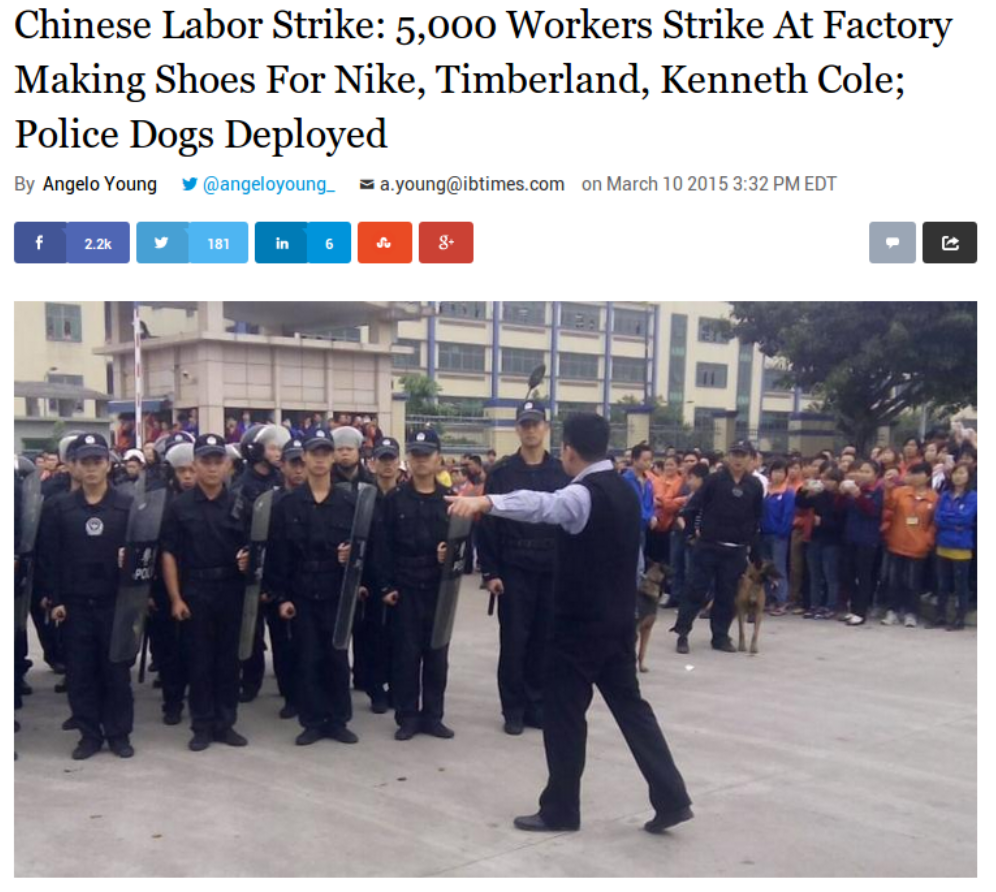
\includegraphics{police_dogs.png}
  \end{figure}
\end{frame}
%--------------------------------------

%--------------------------------------
\begin{frame}
  Labour standards refer to all issues directly affecting workers
  \begin{itemize}
    \item Health and safety in Bangladesh, housing payment in China, minimum wage in South Africa
  \end{itemize}
  \medskip
  Global agreements on labour requires comparison of labour (and salary) standards across countries.
  These standards are generally not directly addressed in trade agreements.
  \begin{itemize}
    \item WTO does not deal with labour standards; International Labour Organisation is relevant body
  \end{itemize}
\end{frame}
%--------------------------------------

%--------------------------------------
\begin{frame}
 Internationally regulated living wage is controversial as it is difficult to compare labour standards across countries
 \begin{itemize}
   \item Low wages are comparative advantage: risk of increased unemployment as higher wages mean less demand
 \end{itemize}
 \medskip
 Does not entail that other labour standards should be neglected.
\end{frame}
%--------------------------------------

%--------------------------------------
\begin{frame}
Labour standards are basically a list of conventions and recommendations established by the International Labour Organisation (ILO).
There are four main convention areas
\begin{enumerate}
  \item Freedom of association
  \item Abolition of forced labour
  \item Equality
  \item Elimination of child labour  
\end{enumerate}
\end{frame}
%--------------------------------------

%--------------------------------------
\begin{frame}
  \begin{figure}
    
\includegraphics[scale=.2]{nutella.png}
  \end{figure}
\end{frame}


%--------------------------------------
\begin{frame}
  Improving labour conditions is often a slow process, and some argue that trade policy can be used to speed up the process.
  \begin{itemize}
   \item Trade is the only tool there is and it is wrong to benefit from the abuse of others.
  \end{itemize}
  \medskip
  However, although most agree that labour standards should be promoted there is disagreement about whether trade policy is the right tool.
  \begin{itemize}
    \item Trade restrictions will make countries poorer and could provice incentives for protectionism
  \end{itemize}
\end{frame}
%--------------------------------------

%--------------------------------------
\begin{frame}
  \begin{figure}
    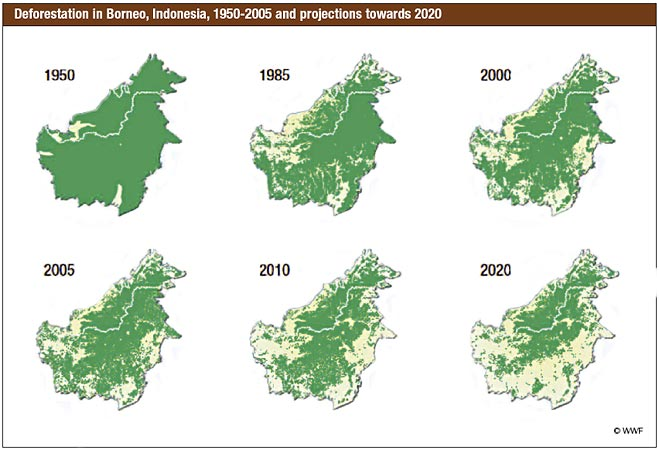
\includegraphics[scale=.4]{borneo.png}
  \end{figure}
\end{frame}
%--------------------------------------

%--------------------------------------
\begin{frame}
 Some concerns concerning trade and the environment
 \begin{enumerate}
   \item Increase in emissions due to transport of goods
   \item Creation of pollution havens
   \item Depletion of international natural resources due to lack of regulations
 \end{enumerate}
\end{frame}
%--------------------------------------

%--------------------------------------
\begin{frame}
  There are two main hypotheses linking trade and the environment
  \begin{enumerate}
    \item Pollution haven hypothesis: Being able to pollute is a comparative advantage
    \item Factor endowment hypothesis: Rich countries will be dirtier due to polluting relatively capital-intensive industries
  \end{enumerate}
\end{frame}
%--------------------------------------

%--------------------------------------
\begin{frame}
 Trade affects the environment in three ways
 \begin{enumerate}
   \item Scale of economic activity: More trade means more production means more pollution
   \item Level of income: Higher income means demand for cleaner production
   \medskip
   \item Composition of output: Trade will alter output composition, based on comparative advantage
 \end{enumerate}
 \medskip
 The scale and technique effect are indirect whereas the composition effect is direct.
\end{frame}
%--------------------------------------

%--------------------------------------
\begin{frame}
  The composition effect has two opposite predictions
  \begin{enumerate}
    \item Pollution haven: Poor countries more polluted, rich countries less
    \item Factor endowment: Poor countries less polluted, rich countries more
  \end{enumerate}
\end{frame}
%--------------------------------------

%--------------------------------------
\begin{frame}
  The main problem of trade in context of the environment is that it generates externalities
  \begin{itemize}
    \item Some costs are not borne by the producer/consumer
    \item e.g. pollution, global warming, extinction of species
  \end{itemize}
\end{frame}
%--------------------------------------

%--------------------------------------
\begin{frame}
  One example of negative externalities is the pollution along the Mexican border, caused by production of goods for US market.
  \begin{itemize}
    \item Stimulated by 'maquiladoras' which are firms given a special tariff treatment carrying out production for US firms
  \end{itemize}
  \medskip
  In another case the US tried to implement some laws to curtail some negative effects such as banning imports from Mexico of tuna and shrimps
  \begin{itemize}
    \item Since this hurt the dolphin and turtle population
  \end{itemize}
  \medskip
  These laws were struck down by the WTO
\end{frame}
%--------------------------------------

%--------------------------------------
\begin{frame}
  There are a number of ways to deal with negative externalities
  \begin{enumerate}
    \item Regulate by prohibiting or limiting activity
    \item Taxation by making the activity more costly
    \item Or a hybrid form such as tradable licenses
    \begin{itemize}
      \item Number of licenses is set up by regulator and market determines who uses one
      \item Cap and trade
    \end{itemize}
  \end{enumerate}
\end{frame}
%--------------------------------------

%--------------------------------------
\begin{frame}
 Economically speaking there is an optimal level for a negative externality which isn't zero. 
 Instead, reducing the externality the optimal level is found when 
 \begin{align*}
   marginal\; benefit = marginal\; cost
 \end{align*}
 \begin{figure}
   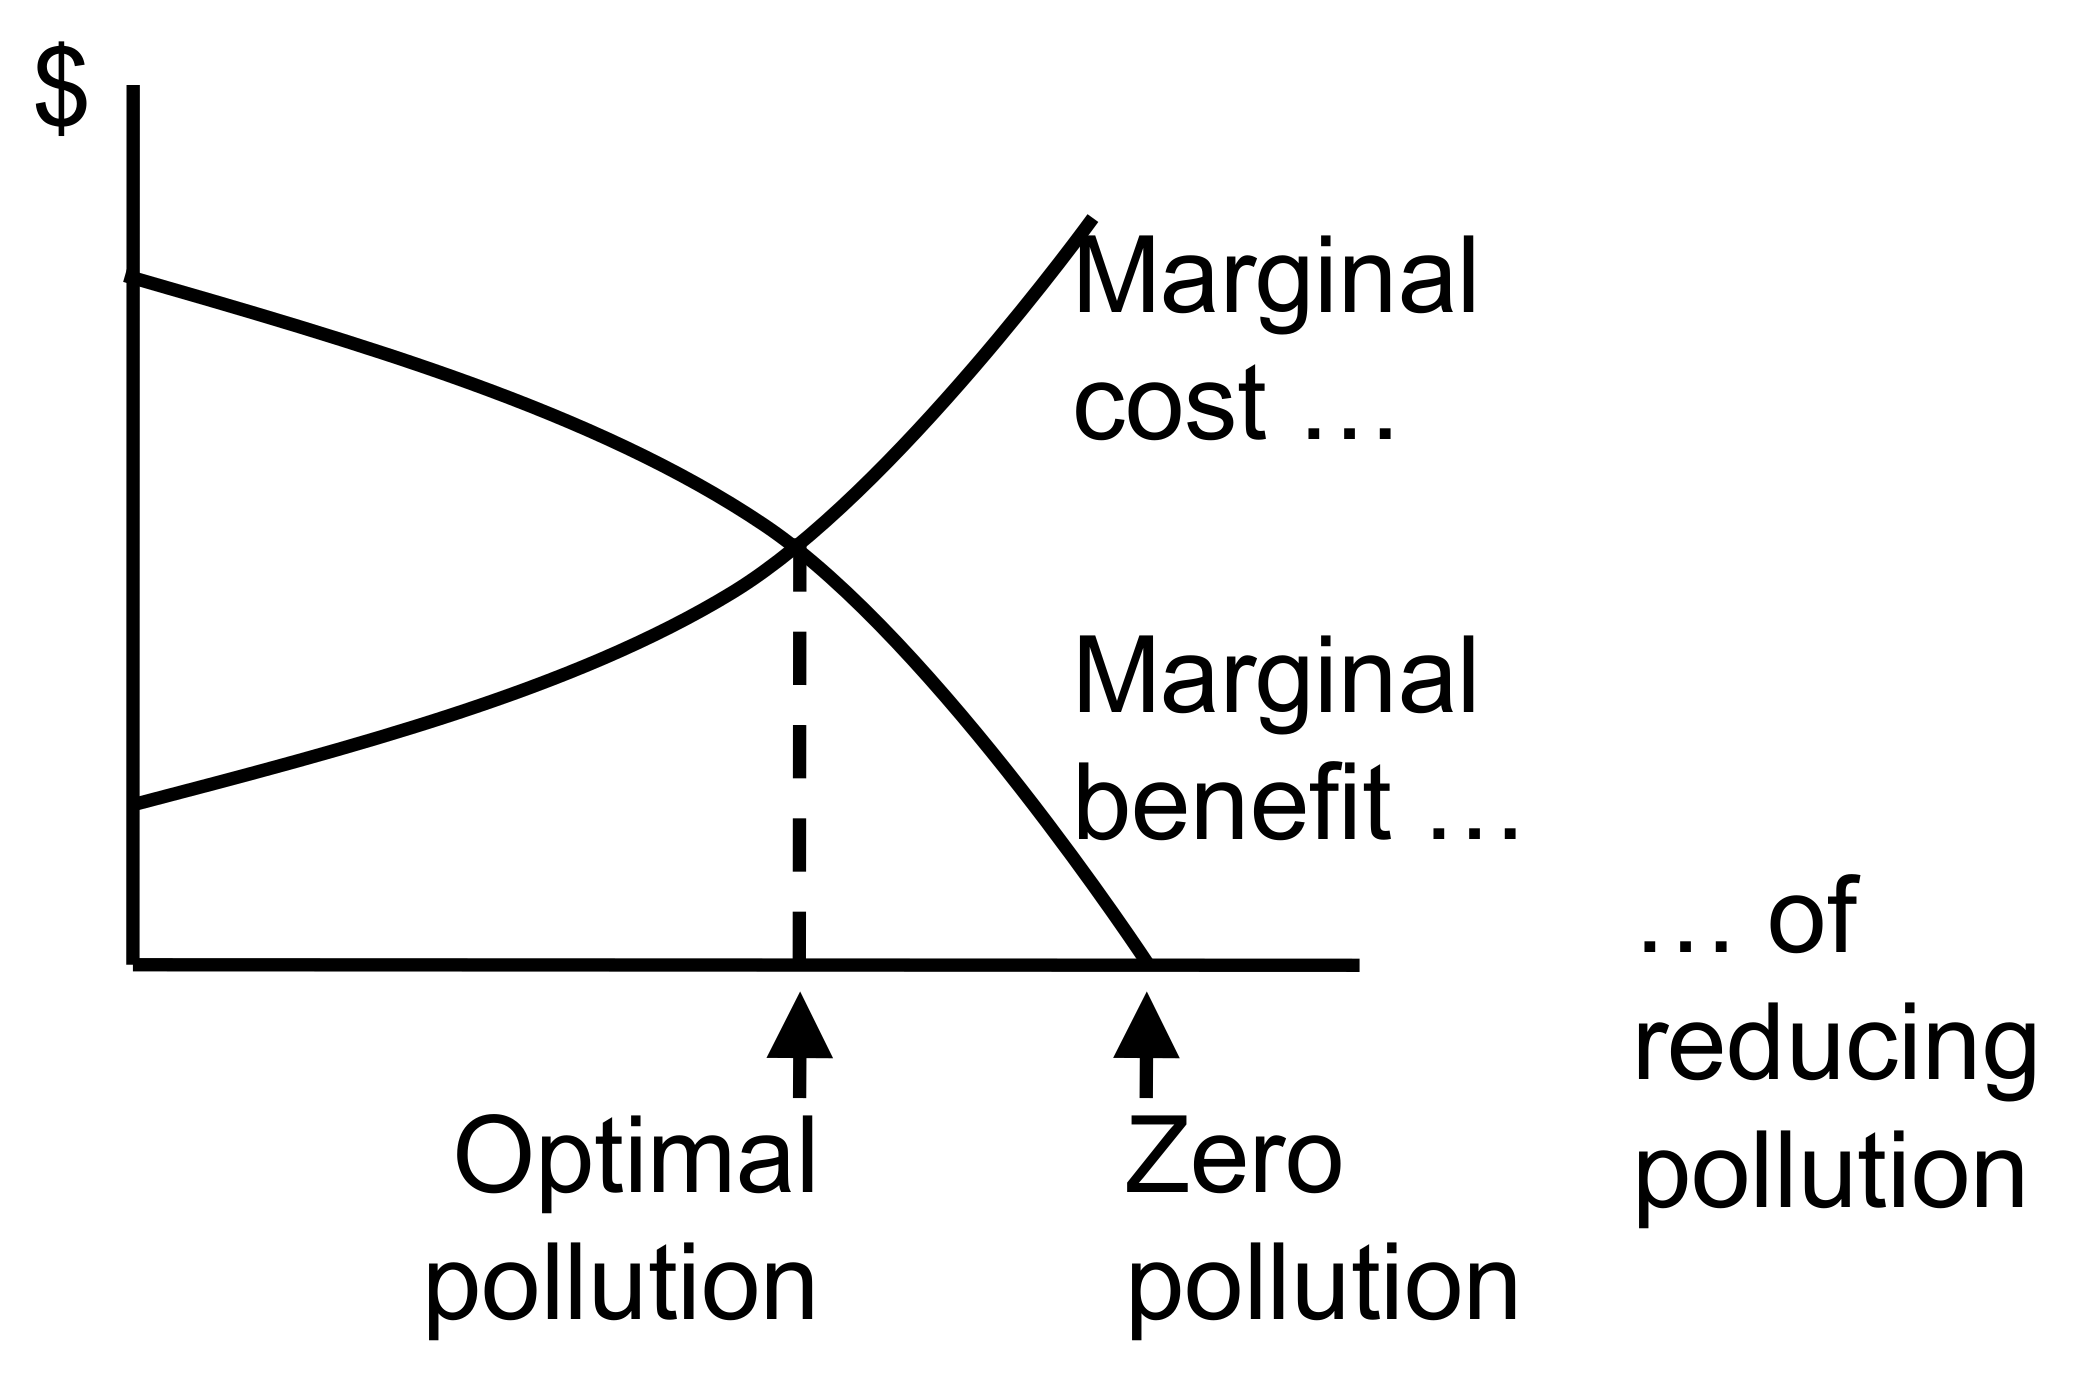
\includegraphics[scale=.3]{externality.png}
 \end{figure}
 \end{frame}
%--------------------------------------

%--------------------------------------
\begin{frame}
 Some more examples of negative externalities
 \begin{itemize}
   \item Pollution of air and water
   \item Acid rain
   \item Global warming, due to $CO_2$ and $MH_4$ emissions
   \item Deforestation, specifically tropical forests in Brazil and Indonesia
   \item Destruction of species
   \item Overuse of natural resources 
 \end{itemize}
\end{frame}
%--------------------------------------

%--------------------------------------
\begin{frame}
  Externalities are often international problems, which makes them hard to solve
  \begin{itemize}
    \item No incentive to incur local costs to limit harm to foreigners
  \end{itemize}
  \medskip
  Needs international agreements
  \begin{itemize}
    \item Choroflorocarbons that caused the hole in the ozone layer were dealt with by the 1987 Montreal protocol
  \end{itemize}
\end{frame}
%--------------------------------------

%--------------------------------------
\begin{frame}
  Regulations are sometimes difficult to implement as it will affect competitiveness. 
  \begin{itemize}
    \item A pollution tax for example will raise costs of exports    
  \end{itemize}
  \medskip
  When countries have weak regulations they can become pollution havens.
  There is a race to the bottom where countries compete by lowering environmental standards
\end{frame}
%--------------------------------------

%--------------------------------------
\begin{frame}
  \begin{figure}
    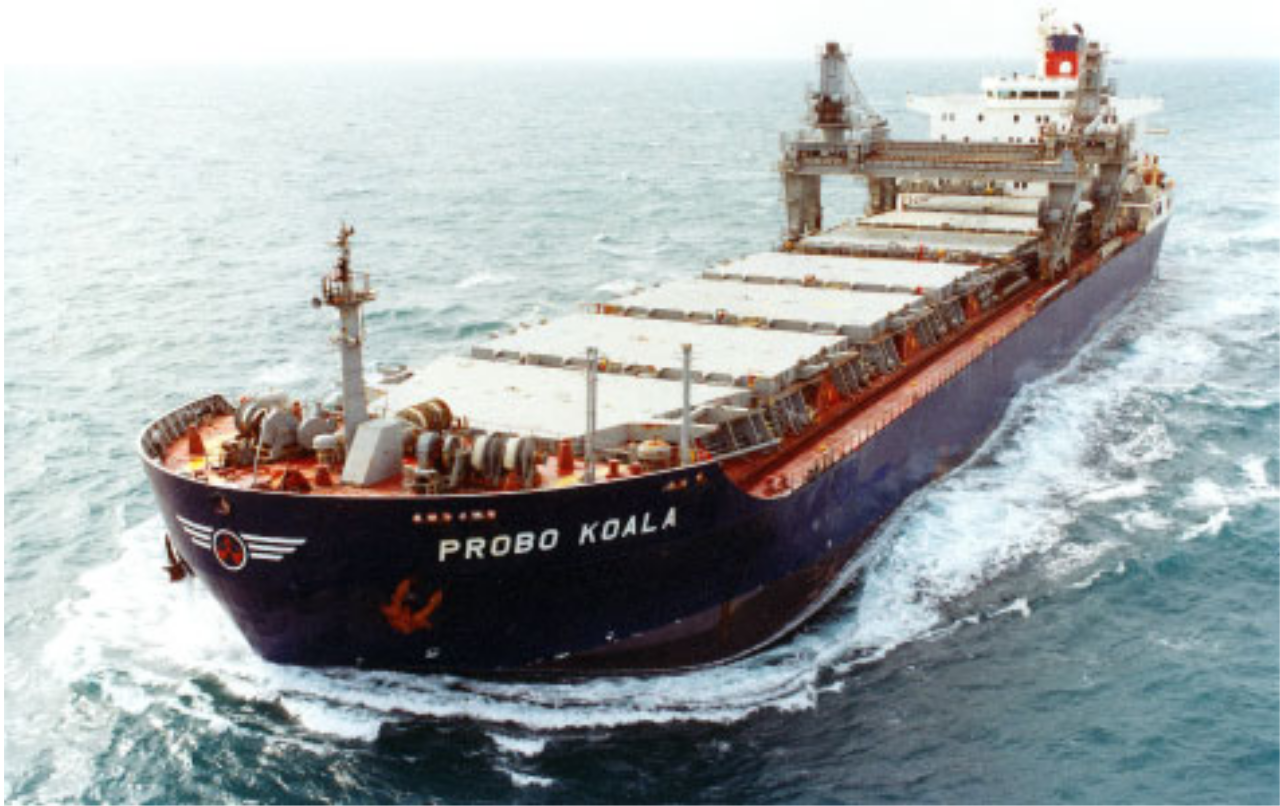
\includegraphics{probo_koala.png}
  \end{figure}
\end{frame}
%--------------------------------------

%--------------------------------------
\begin{frame}
  Following the pollution haven hypothesis low standards are a comparative advantage.
  \begin{itemize}
    \item When pollution control costs start to matter for some industries in some countries, other countries gain comparative advantage in those industries
  \end{itemize}
  \medskip
  This difference in environmental standards will affect the allocation of investments
  \begin{enumerate}
    \item In developing countries production and exports will become more pollution intensive
    \item Pollution-intensive industries will leave high-standard countries
  \end{enumerate}
  \medskip
  Empirically little evidence for this theory.
\end{frame}
%--------------------------------------

%--------------------------------------
\begin{frame}
  \begin{figure}
    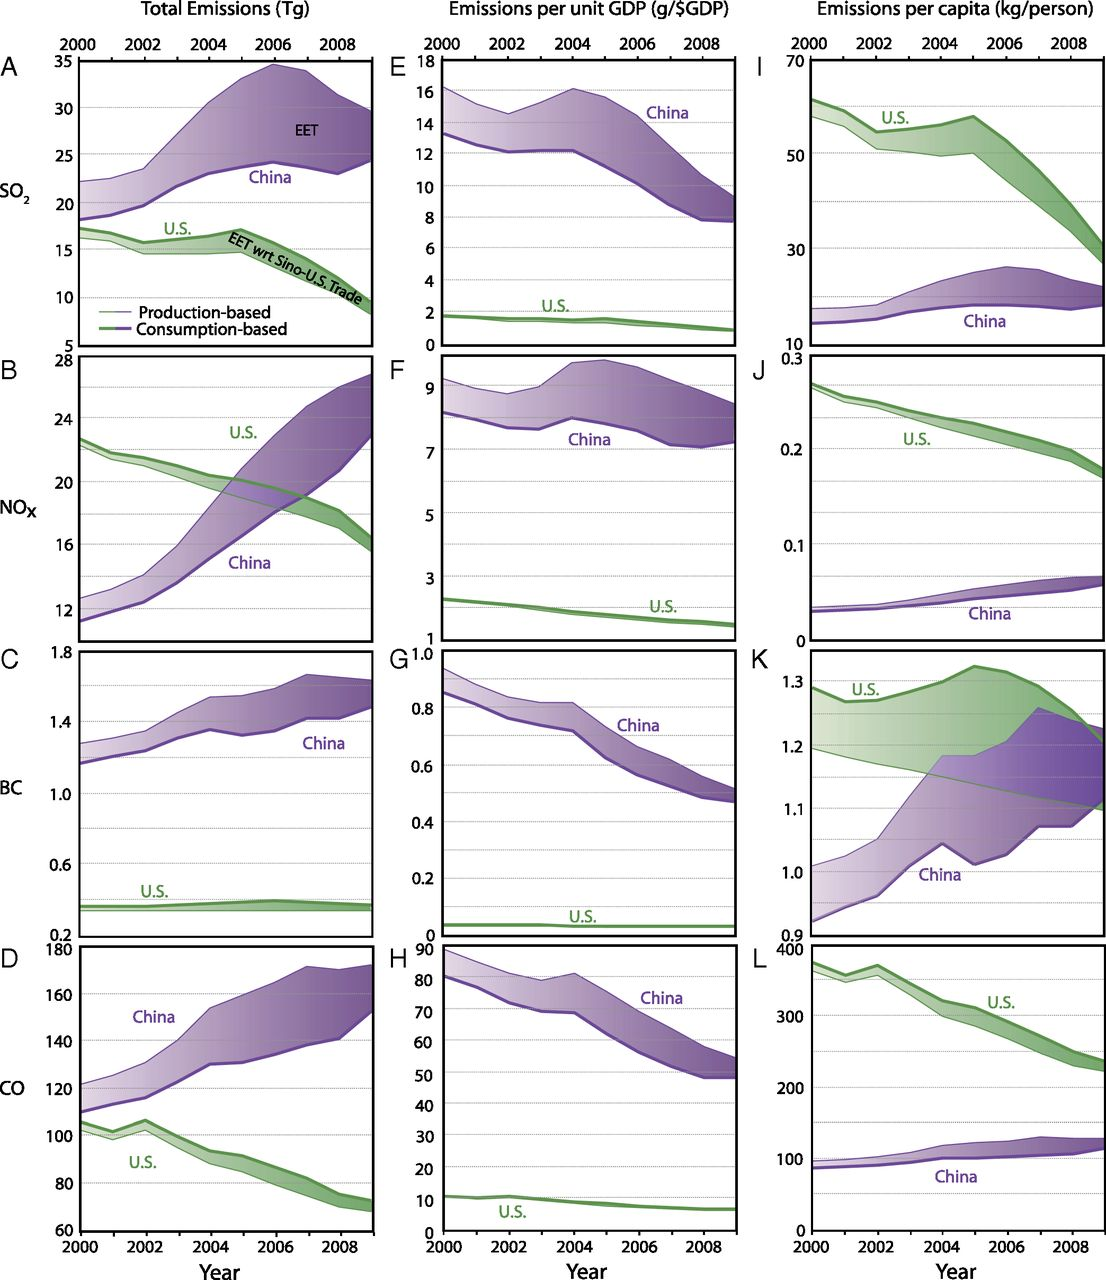
\includegraphics[scale=.7]{emission.png}
  \end{figure}
  "China's international trade and air pollution in the United States"
\end{frame}
%--------------------------------------

%--------------------------------------
\begin{frame}
  The optimal policy depends on the country income's level as poor countries can't afford strict regulations
  \begin{itemize}
    \item The environment is income elastic, meaning that demand increases with income
  \end{itemize}
\end{frame}
%--------------------------------------

%--------------------------------------
\begin{frame}
  \begin{figure}
    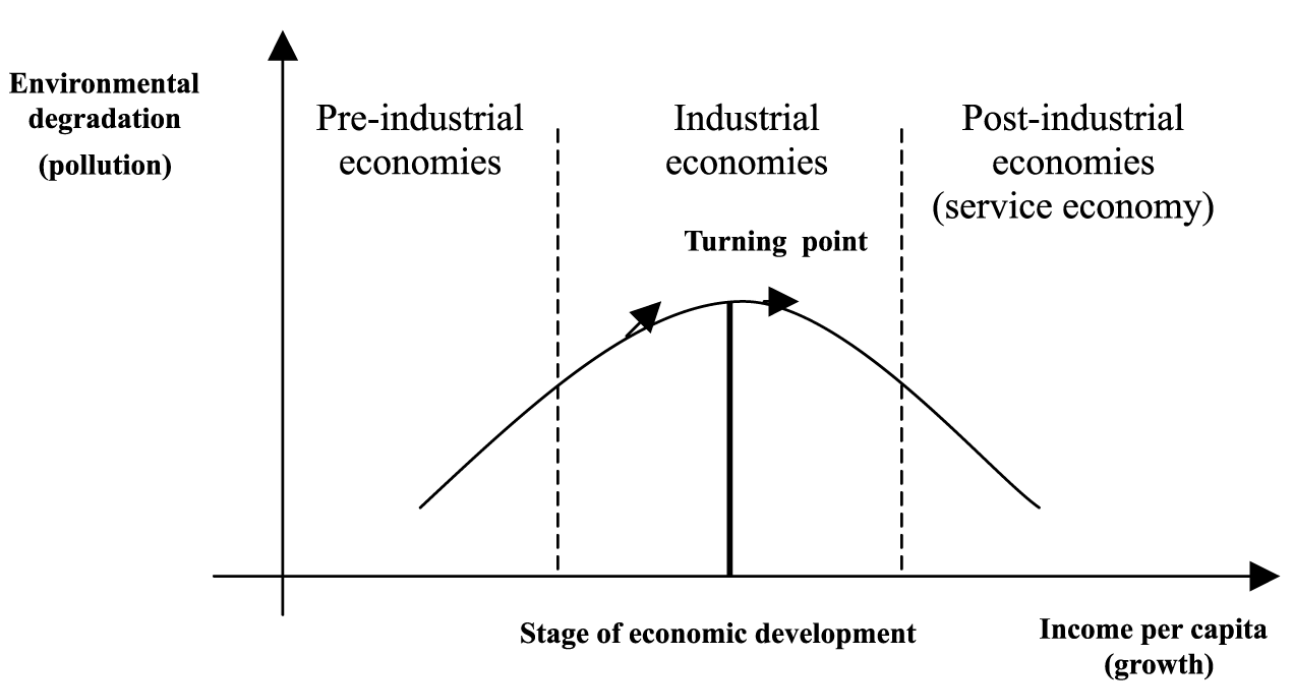
\includegraphics{kuznets.png}
  \end{figure}
\end{frame}
%--------------------------------------

\begin{frame}
  Two channels through which trade and the environment are linked
  \medskip
  \begin{enumerate}
    \item Statically, for a given level
    \begin{itemize}
      \item Race to the bottom in national regulation 
    \end{itemize}
    \item Dynamically, via income growth
    \begin{itemize}
      \item Shift to cleaner techniques and composition of economic activity
    \end{itemize}
  \end{enumerate}
\end{frame}
%--------------------------------------

%--------------------------------------
\begin{frame}
 \textbf{From first lecture:} Mexico is the world’s largest exporter of fresh
tomatoes; which country is the second largest?
\end{frame}
%--------------------------------------

%--------------------------------------
\begin{frame}
  \begin{figure}
    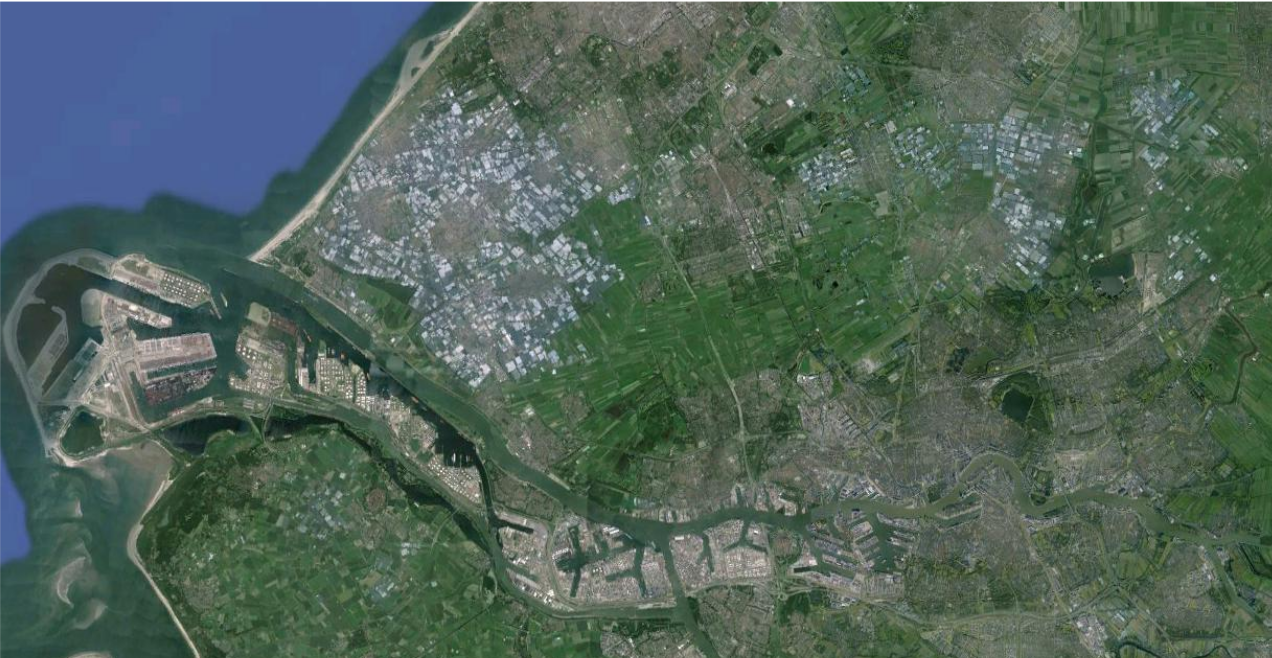
\includegraphics{westland.png}
  \end{figure}
\end{frame}
%--------------------------------------

%--------------------------------------
\begin{frame}
 Does the WTO allow limits on imports concerning environmental reasons?
 \begin{itemize}
   \item Yes, if the imported goods do damage inside the importing countries
   \item No, if the damage is done in the exporting country or abroad
 \end{itemize}
 \medskip
 Recall that policy does not allow discrimination, as such imports may not be limited based on the production process.
\end{frame}
%--------------------------------------

%--------------------------------------
\begin{frame}
 An example of a policy designed to discourage harmful production methods is the so called carbon tariff: These tariffs are implemented to limit CO$_2$ emissions, but not applied by all countries
 \begin{itemize}
   \item This kind of tariffs aims to rise the price of carbon
 \end{itemize}
 \medskip
 Some countries don't participate: could put tariff on exports of non-participating countries.
 \begin{itemize}
   \item Benefits to the world are the same but the costs are not
 \end{itemize}
\end{frame}
%--------------------------------------

%--------------------------------------
\begin{frame}
 There are arguments for and against using this type of tariff
 \begin{itemize}
   \item Carbon tariff is protectionist and imposing them would lead to trade wars   
   \medskip
   \item Not implementing this tariff would lead to consumer substitution towards products made in countries that do not tax/restrict CO$_2$ emissions
   \begin{itemize}
     \item Can be implemented under WTO rules as border tax adjustments   
   \end{itemize}   
 \end{itemize}
\end{frame}
%--------------------------------------

%--------------------------------------


%--------------------------------------
\begin{frame}
  \textbf{Tragedy of the commons} (Hardin, 1968)
  \begin{quote}
    The population problem has no technical solution; it requires a fundamental extension in morality
  \end{quote}
\end{frame}
%--------------------------------------

%--------------------------------------
\begin{frame}
  With common we generally mean a resource that is owned jointly
  \begin{itemize}
    \item e.g. the oceans, but also extractive industries
  \end{itemize}
  \medskip
  Although the benefits of using the resource are acrued individually, the costs are borne jointly
  \begin{itemize}
    \item The individual cost is therefore reduced
  \end{itemize}
  \medskip
  The imbalance between cost and benefit makes increasing exploitations a rational strategy; this will lead to overexploitation.
\end{frame}
%--------------------------------------

%--------------------------------------
\begin{frame}
 Hardin illustrated the tragedy of the commons using a open pasture which can be used by herdsmen for their cattle.
 \begin{itemize}
   \item Expectation is that each herder will try to keep as much cattle as possible
 \end{itemize}
 \medskip
 This strategy will work as long as other factors keep the population below the carrying capacity of the land until social stability is reached. 
 Things will go pear-shaped when herders will try to maximise utility
 \begin{enumerate}
   \item Each herder will add one more animal to herd which gives positive utility of +1
   \item Extra animal will lead to overgrazing with utility of -1, shared by all herdsmen
 \end{enumerate}
 \medskip
 This will lead to a theoretically unlimited increase on a limited resource.
\end{frame}
%--------------------------------------

%--------------------------------------
\begin{frame}
  \begin{figure}
    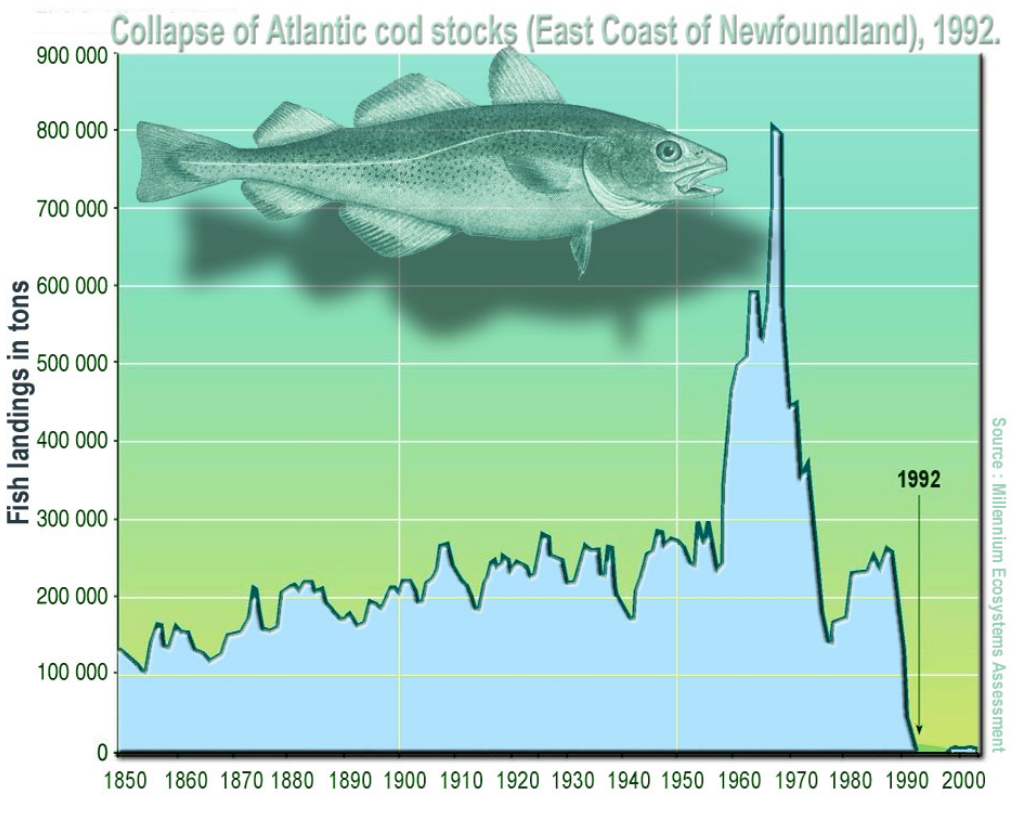
\includegraphics{cod.png}
  \end{figure}
\end{frame}
%--------------------------------------

%--------------------------------------
\begin{frame}
  There are a number of ways to manage the commons such as
  \begin{enumerate}
    \item Converting it into private property
    \item Allocating rights to using the commons
    \item Coercion
  \end{enumerate}
  \medskip
  Some of these are hard to apply at international level
\end{frame}
%--------------------------------------

%--------------------------------------
\begin{frame}
  \begin{figure}
    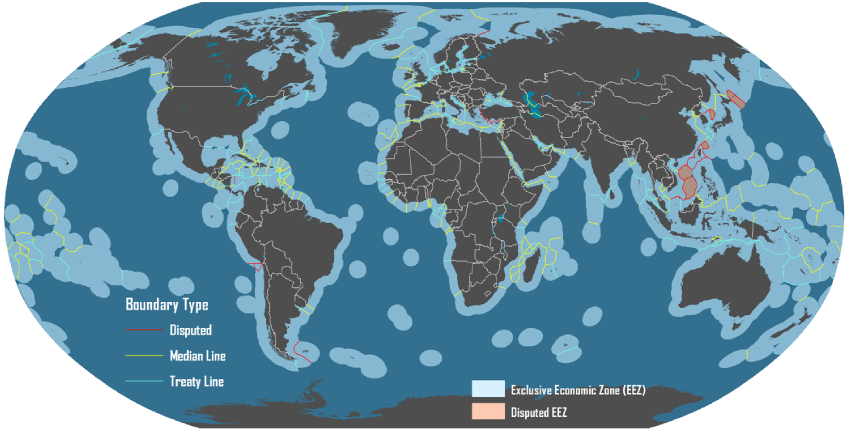
\includegraphics[scale=.5]{EEZ.png}
  \end{figure}
\end{frame}
%--------------------------------------

%--------------------------------------
\begin{frame}
  The tragedy of the commons is a so called no technical solutions problem.
  \begin{itemize}
    \item Instead it requires a change in morality of human values
  \end{itemize}
  \medskip
  This is because rational actors will continue to exploit the commons.
  \begin{itemize}
    \item Therefore a change in values is needed which makes exploiting the resource past carrying-capacity no longer rational
  \end{itemize}
\end{frame}
%--------------------------------------

%% FIN
%------------------------------------------------------------------------------
\end{document}
